\begin{frame}{5G - Network Function functionalities}
  Network Functions can perform:
  \begin{itemize}
  \item<1-> Packet elaboration
  \item<2-> Deep Packet Inspection
  \item<3-> Firewalling
  \item<4-> Header enrichment
  \item<5-> Compression
  \item<6-> Traffic Layer optimization
  \item<7-> \dots
  \end{itemize}

  % ... and how you can imagine all the mentioned network function, deployed in
  % a hardwarized manner can be a hell to manage
  \begin{textblock*}{5cm}(1.25cm,1.4cm)
    \begin{itemize}
      \item[]<8-> 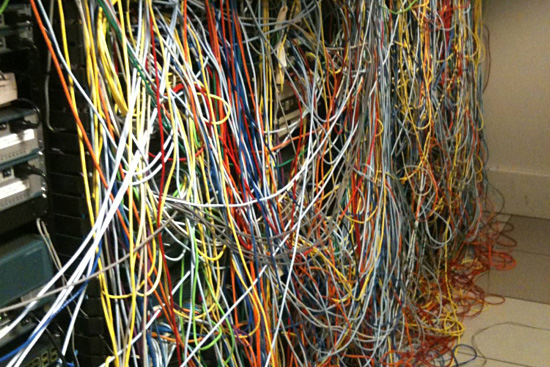
\includegraphics[scale=0.5]{server_spaghetti}
    \end{itemize}
  \end{textblock*}
\end{frame}

\begin{frame}{5G - \textit{Virtual} Network Function}
  \begin{itemize}
    \item[]<1-> Why don't we go ``virtual''?
  \end{itemize}

  \begin{itemize}
  \item[]<2-> Benefits:
    \begin{itemize}
    \item<3-> Less maintenance costs
    \item<4-> Less time to deploy
    \item<5-> More flexibility
    \item<6-> Automation
    \end{itemize}
  \end{itemize}


  %\begin{textblock*}{5cm}(0.5cm,5cm)
  %  \begin{itemize}
  %  \item[]<1-> \includegraphics[scale=0.4]{team_chat}
  %  \end{itemize}
  %\end{textblock*}

  % And how do we go virtual? Well, we have different solutions and approach,
  % for example we have container-based virtualization technologies or
  % hypervisor-based one.
  \begin{textblock*}{5cm}(1.5cm,1.2cm)
    \begin{itemize}
    \item[]<2-> 
\includegraphics[scale=0.25]{docker_logo}
    \end{itemize}
  \end{textblock*}

  \begin{textblock*}{5cm}(7.2cm,1.2cm)
    \begin{itemize}
    \item[]<3-> 
\includegraphics[scale=1.4]{virtualbox_logo}
    \end{itemize}
  \end{textblock*}

  \begin{textblock*}{5cm}(6cm,3cm)
    \begin{itemize}
    \item[]<6-> 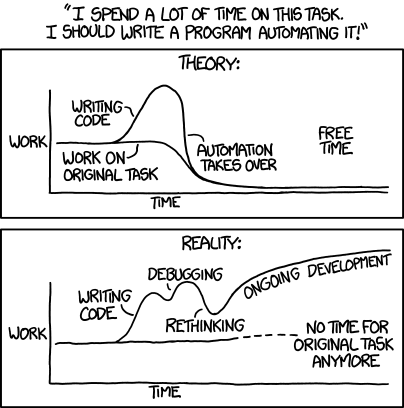
\includegraphics[scale=0.4]{automation}
    \end{itemize}
  \end{textblock*}
\end{frame}
